%; whizzy paragraph -pdf xpdf -latex ./whizzypdfptex.sh
%; whizzy-paragraph "^\\\\begin{frame}\\|\\\\emtext"
% latex beamer presentation.
% platex, latex-beamer でコンパイルすることを想定。 

%     Tokyo Debian Meeting resources
%     Copyright (C) 2012 Junichi Uekawa
%     Copyright (C) 2016 Nobuhiro Iwamatsu

%     This program is free software; you can redistribute it and/or modify
%     it under the terms of the GNU General Public License as published by
%     the Free Software Foundation; either version 2 of the License, or
%     (at your option) any later version.

%     This program is distributed in the hope that it will be useful,
%     but WITHOUT ANY WARRANTY; without even the implied warreanty of
%     MERCHANTABILITY or FITNESS FOR A PARTICULAR PURPOSE.  See the
%     GNU General Public License for more details.

%     You should have received a copy of the GNU General Public License
%     along with this program; if not, write to the Free Software
%     Foundation, Inc., 51 Franklin St, Fifth Floor, Boston, MA  02110-1301 USA

\documentclass[cjk,dvipdfmx,12pt]{beamer}
\usetheme{Tokyo}
\usepackage{monthlypresentation}

%  preview (shell-command (concat "evince " (replace-regexp-in-string "tex$" "pdf"(buffer-file-name)) "&")) 
%  presentation (shell-command (concat "xpdf -fullscreen " (replace-regexp-in-string "tex$" "pdf"(buffer-file-name)) "&"))
%  presentation (shell-command (concat "evince " (replace-regexp-in-string "tex$" "pdf"(buffer-file-name)) "&"))

%http://www.naney.org/diki/dk/hyperref.html
%日本語EUC系環境の時
\AtBeginDvi{\special{pdf:tounicode EUC-UCS2}}
%シフトJIS系環境の時
%\AtBeginDvi{\special{pdf:tounicode 90ms-RKSJ-UCS2}}

\newenvironment{commandlinesmall}%
{\VerbatimEnvironment
  \begin{Sbox}\begin{minipage}{1.0\hsize}\begin{fontsize}{8}{8} \begin{BVerbatim}}%
{\end{BVerbatim}\end{fontsize}\end{minipage}\end{Sbox}
  \setlength{\fboxsep}{8pt}
% start on a new paragraph

\vspace{6pt}% skip before
\fcolorbox{dancerdarkblue}{dancerlightblue}{\TheSbox}

\vspace{6pt}% skip after
}
%end of commandlinesmall

\title{東京エリアDebian勉強会\\Debian JP Project}
\subtitle{OSC 2018 Tokyo/Fall (第167回出張勉強会)}
\author{杉本 典充\\ dictoss@live.jp}
\date{2018年10月27日}
\logo{
\includegraphics[width=8cm]{image200607/openlogo-light.eps}}

\begin{document}

\section{表紙}

\begin{frame}
\titlepage{}
\end{frame}

\section{目次}

\begin{frame}{Agenda}
  \begin{itemize}
  \item Debian とは?
  \item Debian JP Project と Debian 勉強会
  \item Debian 9 (Stretch)
  \item Debian Updates
  \item 今後のイベント
  \end{itemize}
\end{frame}

%-------------------

\section{Debian とは?}

\begin{frame}\begin{center}\Huge{Debian とは?}\end{center}\end{frame}


\begin{frame}{Debian とは?}

{\color{red}{フリー/オープン}}な{\color{red}{ユニバーサル}}オペレーティングシステム を作成しようとするボランティアベースのプロジェクト

\begin{table}[htb]
  \begin{tabular}{|c|c|c|}
    \hline
    ディストリ & 企業 & ボランティア \\ \hline
    RHEL & RedHat & なし  \\ \hline
    CentOS & RedHat & あり \\ \hline
    Ubuntu  & Canonical & あり \\ \hline
    \color{red}{Debian}  & \color{red}{なし} & \color{red}{あり} \\ \hline
  \end{tabular}
\end{table}

\end{frame}

\begin{frame}{Debian とは?}
 世界規模で開発が行われており、63ヶ国、約1000名のDebian公式開発者が開発を行
 っている。パッケージメンテナや翻訳などの貢献者も入れるともっと多くの開発者が参加
 していることになる。
 \begin{center}
%%%   \includegraphics[width=0.7\hsize]{image201707/group_photo_t.jpg}
 \end{center}
\end{frame}


\begin{frame}{Debian とは?}

\begin{itemize}
  \item 利用用途
  \begin{itemize}
    \item Linuxサーバ (例:webサーバのシェア:\url{https://w3techs.com/technologies/details/os-linux/all/all})
    \item 組込デバイスのベースOS (多くのCPUで動作する)
    \item デスクトップPC、ノートPCなどの普段利用するコンピュータのOS
  \end{itemize}
  \item 「Debian」ベースな派生OSの源流
  \begin{itemize}
    \item Ubuntu や Raspbian といったディストリビューションのベースはDebian
    \item 派生先のディストリビューションと相互に情報交換をして開発している
  \end{itemize}
\end{itemize}

\end{frame}


\begin{frame}{Debian とは?}

\begin{itemize}
  \item 2018年10月の時点で、最新版は {\color{red}{Debian 9.5}} (コードネーム: Stretch)
  \begin{itemize}
    \item パッケージ数は{\color{red}{約51000}}を提供
    \item 公式にサポートするCPUアーキテクチャは{\color{red}{10}}
  \end{itemize}
  \item {\color{red}{約2年毎}}にリリース
  \item 次のリリース Debian 10 (コードネーム: {\color{red}{}}Buster)は 2019年中頃にリリースすると思われる
  \item コードネームはトイ・ストーリーのキャラクターを採用
\end{itemize}

\end{frame}


\begin{frame}{Debian とは?}

\begin{itemize}
  \item Debian 社会契約
    \begin{itemize}
      \item Debian 開発者たちが目指すフリーソフトウェアコミュニティーの在り方
    \end{itemize}
  \item Debian フリーソフトウェアガイドライン(DFSG)
    \begin{itemize}
      \item Debian 社会契約の一部
      \item Debian が考えるフリーソフトウェアの定義
      \item オープンソースの定義のひな形にもなっている
    \end{itemize}
  \item Debian Policy
    \begin{itemize}
      \item \url{https://www.debian.org/doc/debian-policy/}
      \item Debian パッケージの区分、内容やルール、ファイル配置の方針を定義
    \end{itemize}
\end{itemize}

\end{frame}


\if 0
\begin{frame}{Debian とは?}
  \begin{center}
%  \includegraphics[width=0.5\hsize]{image201611/chin_.jpg}
% buz の顎拡大画像
  \end{center}
\end{frame}

\begin{frame}{Debian とは?}
どこで使われているのか?\pause
Linux ディストリビューションのベース

  \begin{center}
%   \includegraphics[width=0.5\hsize]{image201606/ubuntu.png}
  \end{center}

\end{frame}

\begin{frame}{Debian とは?}
Webサーバとして利用されてる(2016/06時点)

  \begin{center}
%  \includegraphics[width=0.5\hsize]{image201606/w3techs.png}
  \end{center}
  \tiny{\url{http://w3techs.com/technologies/details/os-linux/all/all}}

\end{frame}

\begin{frame}{Debian とは?}
組込デバイスのベースOSとして利用されている

 \begin{center}
% \includegraphics[width=0.5\hsize]{image201606/bbb-logo.jpeg}
%%  http://www.tech-villa.com/images/kallyas_images/blog_images/beagleboneblack_logo.jpg
 \end{center}
 \url{http://beagleboard.org/}

 \begin{center}
% \includegraphics[width=0.2\hsize]{image201606/rpi-logo.png}
%  https://www.raspberrypi.org/wp-content/uploads/2015/08/raspberry-pi-logo.png
 \end{center}
 \url{https://www.raspberrypi.org/}

 \end{frame}

\begin{frame}{Debian とは?}

\begin{itemize}
\item ISS (国際宇宙ステーション)
\begin{center}
% \includegraphics[width=0.5\hsize]{image201606/STS-134_International_Space_Station_after_undocking}
 https://ja.wikipedia.org/wiki/%E5%9B%BD%E9%9A%9B%E5%AE%87%E5%AE%99%E3%82%B9%E3%83%86%E3%83%BC%E3%82%B7%E3%83%A7%E3%83%B3#/media/File:STS-134_International_Space_Station_after_undocking.jpg
\end{center}
{\tiny \url{https://training.linuxfoundation.org/why-our-linux-training/training-reviews/linux-foundation-training-prepares-the-international-space-station-for-linux-migration}}

\item Steam (ゲームPC OS)
\item NAS、ルータ
\item etc..
\end{itemize}

\end{frame}

\fi


\begin{frame}{Debian とは?}
まとめると
\begin{itemize}
  \item Debianはフリー/オープンなオペレーティングシステム (OS)を作成しようとするボランティアベースのプロジェクト
  \item 自分たちの考えるフリーという言葉に関する定義、開発目的、パッケージングポリシーを厳格に決めている
  \item 世界中に1000人以上の開発者がおり、他のディストリビューションのベースとして採用されている
  \item 約2年毎にリリースが行われ、多くのパッケージとアーキテクチャをサポートしている
  \item 上記のような特徴から様々なところで利用されているLinuxディストリビューション
\end{itemize}

\end{frame}

%------------------


\section{Debian JP Project と Debian勉強会}


\begin{frame}
  \begin{center}\Huge{Debian JP Project\\と\\Debian勉強会}\end{center}
\end{frame}

  
\begin{frame}{Debian JP Project とは?}

\begin{itemize}
  \item 日本でDebianを普及させることを目的とした任意団体
  \item 活動内容
  \begin{itemize}
    \item Debian の日本語による情報発信
    \item ユーザとの情報交換
    \item Debian 開発者、パッケージメンテナの育成など
  \end{itemize}
\end{itemize}

\end{frame}


\begin{frame}
  
\frametitle{Debian勉強会}
\begin{itemize}
 \item 2005年1月開始
 \item Debian Developer 上川さん発起人
\item 東京と関西で月に一回コンスタントに開催しているDebian開発者、ユーザによる勉強会
\end{itemize}

\end{frame}

\begin{frame}

\frametitle{Debian勉強会:解決したい内容}
\begin{itemize}
 \item<1-> 問題
       \begin{itemize}
	\item MLとIRCで情報交換していた
	\item face-to-faceであう場所がない
	\item まとまったドキュメントが出てこない
       \end{itemize}
 \item<2-> Debian勉強会の提案
       \begin{itemize}
	\item 定期的に集まる
	\item 資料を作成する。(GPLで!) \\
	  {\small \url{https://salsa.debian.org/tokyodebian-team/monthly-report}}
       \end{itemize}
\end{itemize}

\end{frame}

\begin{frame}
 \frametitle{Debian勉強会:実際}
 \begin{itemize}
  %\item Debian Weekly News Quiz
  \item Debian 界隈やパッケージング関連の話題など専門の人に話を聞く
  \item Debianで気になった事柄を調べてレポートする
  \item 前回の内容(東京 9月):\\
	\begin{itemize}
	\item 場所: 朝日ネットさん
    \item 「Rethinking of debian/watch rule」(@kenhys)
    \item busterに向けた日本語環境のタスク整理 \url{https://tokyodebian-team.pages.debian.net/2018-09_tokyodebian_langja_bof.txt}
	\end{itemize}
  \item 各地のイベントでDebian普及活動
	\begin{itemize}
      \item OSC2018北海道、OSC2018京都、OSC2018東京
      \item 関西オープンフォーラム
	  \item Debian/Ubuntu ユーザミートアップ in 札幌
	\end{itemize}
 \end{itemize}
\end{frame}

%-----------------------

\section{Debian 9 (Stretch) について}

\begin{frame}
  \begin{center}\Huge{Debian 9 (Stretch) について}\end{center}
  %\begin{center}\Huge{Debian 9 (Stretch)\\リリースおめでとう!}\end{center}
\end{frame}


\begin{frame}{Debian 9 (Stretch) について}% [containsverbatim]

Debian 9 (コードネーム:Stretch)
\begin{itemize}
  \item Debian 9.0は、2017-06-17にリリース
  \item このリリースは、Debian Projectの創始者 Ian Murdock氏に捧げるリリースになっている
% https://www.debian.org/News/2017/20170617
% Ian Murdock, the founder of the Debian project, passed away on 28th December
  % 2015 at his home in San Francisco. He was 42.

  \item 最新のマイナーリリースは Debian 9.5 であり、2018-07-14にリリース

\end{itemize}
  \begin{center}
%%%    \includegraphics[width=0.6\hsize]{image201707/stretch.png}
  \end{center}
\end{frame}


\begin{frame}{Debian 9 について}% [containsverbatim]

サポートアーキテクチャ
\begin{itemize}
\item サポートされるアーキテクチャ \\
  amd64, i386(i686以降), armel, armhf, arm64, mips, mipsel, mips64el, ppc64el, s390x
%\item サポートから外れたアーキテクチャ \\
%  powerpc
\end{itemize}

 \\
サポートされていない移植版として、昔のCPUやRISC-V、FreeBSDやHurdのカーネルを利用したものがある

\small{\url{https://www.debian.org/releases/stable/amd64/release-notes/ch-whats-new.ja.html}}

\end{frame}


\begin{frame}{Debian 9 について}% [containsverbatim]

ソフトウェア
\begin{itemize}
\item Linux カーネルは 4.9
\item ツールチェイン(GCC 6.3.0, binutils 2.28, glibc 2.24), LLVM 3.7.1, 3.8.1, 3.9.1
\item Perl 5.24.1, Python 2.7.13/3.5.3, Ruby 2.3.3, PHP 7.0.19, Go 1.7.4, OpenJDK 8
\item GNOME 3.22, KDE 5.8, Xfce 4.12.3, lxde 0.99.0, lxqt 0.11.1
\item MariaDB 10.1.23, PostgreSQL 9.6.3, sqlite 3.15
\item OpenSSL 1.1.0, GnuPG 2.1.18/1.4.21
\item クロスコンパイラがデフォルトでサポート
\item etc..
\end{itemize}

\end{frame}


\begin{frame}{Debian 9 について}% [containsverbatim]
  \begin{itemize}
  \item 何かおかしい動作や不具合を見つけた場合はバグレポートをお願いします
  \item バグレポートの仕方
    \begin{itemize}
    \item \url{https://www.debian.org/Bugs/Reporting.ja.html}
    \end{itemize}
  \end{itemize}
\end{frame}

%-----------------------

\section{Debian Updates}

\subsection{Timeline}

\begin{frame}
  \begin{center}\Huge{Debian Updates}\end{center}
\end{frame}


\begin{frame}{Debian Updates}% [containsverbatim]

\begin{itemize}
  \item 2017/12/09:  Updated Debian 8.10 released
  \item 2017/12/09:  Updated Debian 9.3  released
  \item 2018/03/10:  Updated Debian 9.4  released
  \item 2018/06/23:  Updated Debian 8.11 released
  \item 2018/07/14:  Updated Debian 9.5  released
\end{itemize}

\end{frame}


\begin{frame}{Debian Updates}% [containsverbatim]

\begin{itemize}
\item 2018/04/18: Debian Project Leader Election 2018 Results\\
\ \\
  \small{2017年のDebian Project Leader(DPL)のChris Lambさんの信任投票となり、信任された。Chrisさんの所信表明は、次のURLで参照できる。\url{https://www.debian.org/vote/2018/platforms/lamby}}

% https://lists.debian.org/debian-devel-announce/2018/04/msg00009.html

\item お得な情報:「Bits from the DPL」\\
\ \\
  \small{月に1回"debian-devel-announce@lists.debian.org"のMLにChrisさんがプロジェクトの進捗を報告している。時間のない方でもこれを読んでおけばDebian Projectの大まかな動きがわかる。}

\end{itemize}

\end{frame}


\begin{frame}{Debian Updates}% [containsverbatim]

\begin{itemize}
\item 2018/05/01: Call for testing openssl TLS 1.3 support\\
\ \\
  \small{OpenSSL 1.1.1からTLS 1.3を利用できるため、テストするように呼び掛けるアナウンスを実施。}

% https://lists.debian.org/debian-devel-announce/2018/05/msg00000.html

%\item 2018/05/02:  autopkgtest results influencing migration from unstable to testing\\
%\ \\
%  \small{調べる}
%
% https://lists.debian.org/debian-devel-announce/2018/05/msg00001.html
  
\end{itemize}

\end{frame}


\begin{frame}{Debian Updates}% [containsverbatim]

\begin{itemize}
\item 2018/5/31:  Alioth shutdown\\
\ \\
  \small{2003年から開発者向けにCMS、リポジトリサーバとして稼働していたalioth.debian.orgが提供終了。後継のsalsa.debian.orgへ機能を引き継いだ。\url{https://salsa.debian.org/public} でgitlabが稼働し、Kubernetes(k8s)と組み合わせたCI/CDも実行可能。}

\end{itemize}

\end{frame}


\begin{frame}{Debian Updates}% [containsverbatim]

\begin{itemize}
\item 2018/06/05:  Data Protection team delegation\\
\ \\
\small{EUで施行されたGDPRに対応するためのチームとメンバーを紹介。アドバイスが欲しい場合はDebian Data Protection teamへ問い合わせることができる。}

% https://lists.debian.org/debian-devel-announce/2018/06/msg00000.html

\end{itemize}

\end{frame}


\subsection{DebConf18}

\begin{frame}
  \begin{center}\Huge{DebConf18}\end{center}
\end{frame}


\begin{frame}{Debian Updates / DebConf18}% [containsverbatim]

\begin{itemize}
    
\item \url{https://debconf18.debconf.org/}
\item 台湾 新竹市(Hsinchu)の國立交通大學で開催
\item アジア地域での開催は初めて
\item DebCamp 2018/7/21 - 7/27
\item OpenDay 2018/7/28
\item DebConf 2018/7/29 - 8/5

\end{itemize}


\includegraphics[scale=1.0]{image201810/DebConf18_Horizontal_Logo.png}

\end{frame}


\begin{frame}{Debian Updates / DebConf18}% [containsverbatim]

\begin{itemize}
\item 各国にいるDebian開発者が集まった
\item 参加者数は、300名を超える人たちが集まった
\end{itemize}

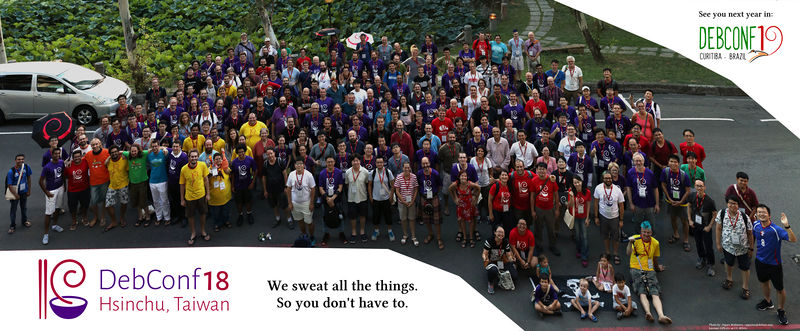
\includegraphics[scale=0.4,bb=0 0 800 331]{image201810/800px-Debconf18_group_photo.jpg}

\end{frame}


\begin{frame}{Debian Updates / DebConf18}% [containsverbatim]

\begin{itemize}
\item セミナー発表はビデオを公開中 \url{https://debconf18.debconf.org/schedule/}
\item 日本から行った人たちがまとめた参加セミナーの情報
  \begin{itemize}
    \item \url{https://tokyodebian-team.pages.debian.net/2018-08_tokyodebian_debconf18_bof.txt}
  \end{itemize}
\end{itemize}

%%%\includegraphics[scale=0.04]{image201810/IMG_4552.JPG}
% https://wiki.debconf.org/wiki/DebConf18/Photos
%  Aigars Mahinovs (aigarius) - Google Photos
%  https://lh3.googleusercontent.com/h6xIiaSy0Yx9XJOnTpzMlaC2_kymnmKfBDTRuNC9Ori8whzxi4nxvizvrFR_XFEHMrE5z1itgyRG-7FRZPaZDnS8DbiRihCloASeeFBCJjKgvjjCV5pSOkWEDZmfkD_NWrfyESoC_uRYG1NjUd2__FvfNZ3VEQ

\end{frame}

\begin{frame}{Debian Updates / DebConf18}% [containsverbatim]

\begin{itemize}
\item セミナー発表のタイトルの一部抜粋
  \begin{itemize}
  \item Bits from the DPL
  \item Debian Science BoF
  \item Ignoring Negativity
  \item News from the APT team
  \item Debian Brasil and DebConf19
  \item Debian Diversity Team discussion session
  \item Report from the Debian EFI team about the support of Secure Boot on Debian
  \item Making Debian more user friendly by changing the web start page (www.debian.org)
  \item GDPR in Debian
  \item Debian Go Packaging Team BoF
  \item The Free Software Foundation, Debian, and the free software movement
  \end{itemize}
\end{itemize}

\end{frame}


\begin{frame}{Debian Updates / DebConf18}% [containsverbatim]

イベント中の生活
\begin{itemize}
  \item Code of Conduct を読み、節度ある生活をする
  \item ベジタリアン、ハラールの方を考慮した食事を用意
  \item 宿泊は学生寮に滞在可能
  \item wikiを読んで行動する \url{https://wiki.debconf.org/wiki/DebConf18}
  \item お知らせはアナウンスメールを読む \url{https://lists.debian.org/debconf-announce/}
  \item セブンイレブン、ファミリーマートが大学構内にあり便利
  \item 大学内のスポーツ施設を有料で利用可能
\end{itemize}

\end{frame}


\begin{frame}{Debian Updates / DebConf18}% [containsverbatim]

ハックラボ
\begin{itemize}
\item 今回はNoisy Hacklab、Quiet Hacklabの2部屋を用意
\item インターネット回線、電源を完備
\item コーヒーやビールを飲みながらハックし、議論し、親交を深める
\end{itemize}

%%%\includegraphics[scale=0.025]{image201810/IMG_4534.JPG}
% https://wiki.debconf.org/wiki/DebConf18/Photos
%  Aigars Mahinovs (aigarius) - Google Photos
%  https://lh3.googleusercontent.com/9GbUR4o1QRMyQ9lMZddRM58rEdnk_cXHx9644-3lYyS_hA7TBHFlc1n1gVVr1M0JsjFd6z6mrFxeIOX9HsrbVSW9IeIPSSQcghzYcv52G7GpbrlfCKUhy6zYWOZx70tA_COa4gJG0yhzIbXTiJJ6eitoSLe9pA
%%%\includegraphics[scale=0.025]{image201810/IMG_5065.JPG}
% https://wiki.debconf.org/wiki/DebConf18/Photos
%  Aigars Mahinovs (aigarius) - Google Photos
%  https://lh3.googleusercontent.com/nEnXBYxds7X6H640WGgiAJmPzoHaVST20KM10eOFdVG4BVqo8gjXEMkn4vT40decm2Sl-fbskds-92tos4MBp6-3s8lAG2yUJ2fd-VCtVA60TD9ZXMiXl4zneZ78I8krbFtGxFFrSuevbjqHoWpQMZrEtJR0eQ

\end{frame}


\begin{frame}{Debian Updates / DebConf18}% [containsverbatim]

DayTrip
\begin{itemize}
\item DebConf中に1日、参加者たちが一緒に出かける企画
\item \url{https://wiki.debconf.org/wiki/DebConf18/DayTrip}
\item 工場見学ツアー、文化施設見学ツアー、お茶会ツアー、台北観光ツアー、自転車でツーリング、川遊び
\end{itemize}

%%%\includegraphics[scale=0.12]{image201810/0801_taipei_1.jpg}
% https://wiki.debconf.org/wiki/DebConf18/Photos
%  Macy- Day trip group photo
%  https://lh3.googleusercontent.com/jnwfbEKoJcPRDn_gSpqxdx8t75FhsMHNKwXUGq75RrNe-7EUDjupBZ4pSqEPqV40yrVp7A1TtDn3ZgWq44HpcZFuVBdLqLAzCgZ8pzXR1QMeqw2F_iglHxs-an-CCp8XRTUdGjTAaE2TJee_8iMFJVkedBY6
%%%\includegraphics[scale=0.16]{image201810/0801_river_4.jpg}
% https://wiki.debconf.org/wiki/DebConf18/Photos
%  Macy- Day trip group photo
%  https://lh3.googleusercontent.com/SqT6u153fNB8ApVeEJe-wyxWeb_Y6XDNcoeYqILGra2uCZ312vhRzLCaq6Wtm_y8xGcAIcCkJ7qA58A6Iu6yog_64p7J49-CYuttE-t_EAYMlvqIvYf2jAlTFobudexvzmdesmb0pb6UY9o80ehzFkLGBQgs

\end{frame}


\begin{frame}{Debian Updates / DebConf18}% [containsverbatim]

チーズ&ワインパーティ
\begin{itemize}
  \item 自分の国のワインとチーズを持ち寄るホームパーティ
  \item 異文化理解や新たな発見をするための交流の場
  \item \url{https://wiki.debconf.org/wiki/DebConf18/CheeseWineBoF}
\end{itemize}

%%%\includegraphics[scale=0.025]{image201810/IMG_4781.JPG}
% https://wiki.debconf.org/wiki/DebConf18/Photos
%  Aigars Mahinovs (aigarius) - Google Photos
%  https://lh3.googleusercontent.com/j6x2pACKhb2nHKDryGkHUUfkpRYTmqKgJEIF5WctZHlZh9IVL6Qh2A-JGl0Q8VYtxIbUtg7-egzC3zCR7MM6R0O7K60UXVHT36YEF2N_CZo4WEo08KWhkitf-GwJ4kzN9XRjyB99cq7FbI4CLjEpP9lM5MkU6g
%%%\includegraphics[scale=0.025]{image201810/IMG_4790.JPG}
% https://wiki.debconf.org/wiki/DebConf18/Photos
%  Aigars Mahinovs (aigarius) - Google Photos
%  https://lh3.googleusercontent.com/R3lP7_Y_3Kz-yc4TeZSyxC5fQM2t0uUHYcUaXoU_NVFmoudpb7hA6aRveE0F9IiPGxZ4II2WDiC1pzmplroScl2oBLQnB38XT08hBoy2z_VzmLqQmihfxK7g24FqG-Ic10N4JmTSsDXITGdAZaccZrW36NInNA

\end{frame}

\begin{frame}{Debian Updates / DebConf18}% [containsverbatim]

カンファレンスディナー

\begin{itemize}
  \item 現地の料理を楽しみながら懇親するディナー
  \item スポンサーの方々から挨拶もあります
\end{itemize}

%%%\includegraphics[scale=0.025]{image201810/IMG_5618.JPG}
% https://wiki.debconf.org/wiki/DebConf18/Photos
%  Aigars Mahinovs (aigarius) - Google Photos
%  https://lh3.googleusercontent.com/7Wp_wU_h0mYRZ4_4ZIf1wy7yOyROR8q0JLoijmSzcLq781Fn64aqRaOSCQgJoXCCHw_4aI8vg_-hdy8k-pwTbrJqk0kR2b1sXaxWxJf23WM5zWij6oCHQCLwzziParHa4KJTmxfsmmNIsKpUwqoXFEvGAzkEjQ
%%%\includegraphics[scale=0.025]{image201810/IMG_5641.JPG}
% https://wiki.debconf.org/wiki/DebConf18/Photos
%  Aigars Mahinovs (aigarius) - Google Photos
%  https://lh3.googleusercontent.com/8EKtU1IYlzzwTitBPxoulswKEdISzFY4Wxbqos1zGpbiw-SPR5kQFRWRrCP1G0bZiNciQCfhE52KJ9EwNcCDbnUOTrzNAnr0f1GLPvCnueWNCYpZH65qP9pso4GlFYic-HbWKMVa7YM9cZtQrkyHxPJQk9YBwA

\end{frame}


\begin{frame}{Debian Updates / DebConf19(予告)}% [containsverbatim]

DebConf19
\begin{itemize}
  \item ブラジル南部のクリチバ市にあるFederal University of Technology(UTFPR)で開催
  \item \url{https://wiki.debian.org/DebConf/19}
\end{itemize}


\includegraphics[scale=1.0]{image201810/dc-19-logo.png}

\end{frame}


\subsection{Release Schedule}

\begin{frame}
  \begin{center}\Huge{Release Schedule}\end{center}
\end{frame}

\begin{frame}{Debian Updates / Release Schedule}% [containsverbatim]

\begin{itemize}
\item 2018/09/30:  Debian 10 (Buster) Release Schedule
  \begin{itemize}
  \item 2019-01-12 - Transition freeze
  \item 2019-02-12 - Soft freeze
  \item 2019-03-12 - Full freeze
  \end{itemize}
\item Debian 10は2019年中頃のリリースになるのではないかと推測

% https://lists.debian.org/debian-devel-announce/2018/09/msg00004.html
\end{itemize}

\end{frame}

%-----------------------

\section{日本語によるDebianの情報}

\begin{frame}\begin{center}\Huge{日本語によるDebianの情報}\end{center}\end{frame}

\begin{frame}{日本語によるDebianの情報}
\begin{itemize}
  \item Debian JP Project \\
      \url{https://www.debian.or.jp}
  \item 東京エリアDebian勉強会\\
      \url{https://tokyodebian-team.pages.debian.net/}
  \item 関西Debian勉強会 \\
      \url{https://wiki.debian.org/KansaiDebianMeeting}
  \item Twitter \\
      \url{@debian_jp}
  %\item G+ コミュニティ \\
  %    \url{https://plus.google.com/u/0/communities/106942835439686570073}
  \item  雑誌 Software Design 技術評論社発行 \\
    「Debian Hot Topics」、GPG関連の記事など(隔月連載)
\end{itemize}
\end{frame}

%----------------

\section{今後のイベント}

\begin{frame}\begin{center}\Huge{今後のイベント}\end{center}\end{frame}

\begin{frame}{今後のイベント}

\begin{itemize}
\item 11/17(土) 第168回東京エリアDebian勉強会
  \begin{itemize}
    \item \url{http://tokyodebian.alioth.debian.org/2018-11.html}
    \item セミナーは検討中
  \end{itemize}
\item 11/9(金)、11/10(土) 関西オープンフォーラム
  \begin{itemize}
    \item \url{https://www.k-of.jp/2018/}
    \item{関西Debian勉強会が出展予定}
  \end{itemize}
\item 11/25(日) 第139関西Debian勉強会
  \begin{itemize}
      % \item 福島区民センター  305号室
      \item \url{https://wiki.debian.org/KansaiDebianMeeting/20181125}
  \end{itemize}
\end{itemize}
\end{frame}

\end{document}

;;; Local Variables: ***
;;; outline-regexp: "\\([ 	]*\\\\\\(documentstyle\\|documentclass\\|emtext\\|section\\|begin{frame}\\)\\*?[ 	]*[[{]\\|[]+\\)" ***
;;; End: ***
